\chapter[Manual de usuario]{
  \label{chp:manualdeusuario}
  MANUAL DE USUARIO
}
\thispagestyle{numberingStyle}
\pagestyle{numberingStyle}


\section{Manual de usario aplicación móvil}

\subsection*{Acceso a la aplicación}
\begin{figure}[H]
\centering
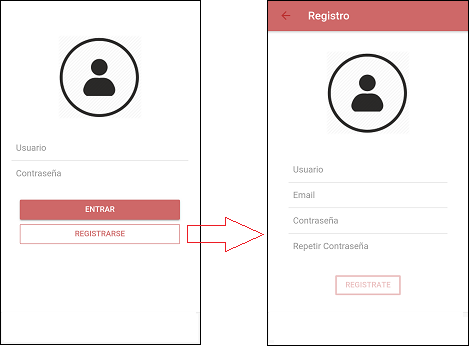
\includegraphics[
   keepaspectratio=true
]{./11_Apendice/Apendice_B/img/Ionic-1-Login.png}
\caption{Pantalla acceso - Aplicación móvil.}
\end{figure}

Cuando se accede a la aplicación por primera vez se mostrará la pantalla que aparece en la parte izquierda de la figura anterior. El usuario, si ya tiene una cuenta registrada, deberá ingresar los datos de acceso y darle al botón de \textit{Entrar} para acceder a la aplicación. Si el usuario no se encuentra registrado deberá registrarse haciendo click sobre el botón \textit{Registrarse}. Al registrarse, se mostrará el formulario que aparece a la derecha en la figura, solicitando los datos de acceso necesarios. El sistema validará los datos de entrada y procederá a la autenticación del usuario.


\subsection*{Pantalla principal}

La pantalla principal de la aplicación estará formada por tres pestañas, que son las siguientes:


\begin{figure}[H]
\centering
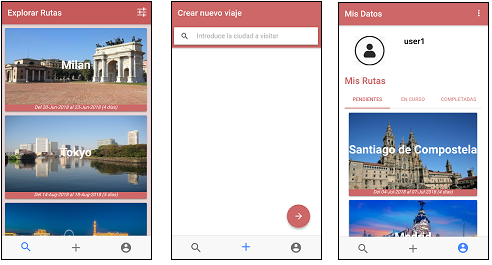
\includegraphics[
   keepaspectratio=true
]{./11_Apendice/Apendice_B/img/Ionic-2-Tabs.png}
\caption{Pantalla acceso - Aplicación móvil.}
\end{figure}

De izquierda a derecha, y mediante el selector que aparece en la parte inferior, se puede alternar entre las pestañas de \textit{Explorar Rutas}, \textit{Crear Ruta} y \textit{Mis Datos}.


\newpage
\subsubsection*{Explorar Rutas}

La pestaña de explorar rutas permitirá poder obtener las rutas de los demás usuarios.

\begin{figure}[H]
\centering
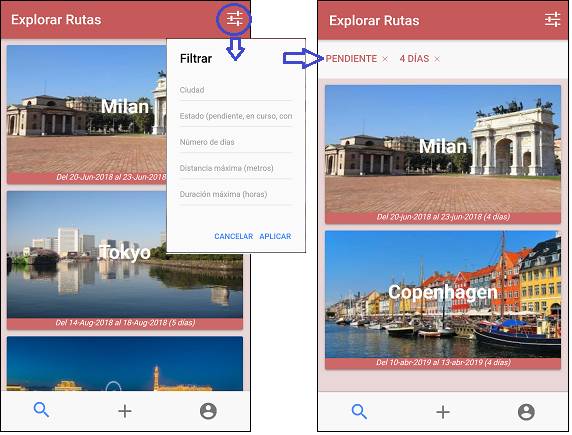
\includegraphics[
   keepaspectratio=true
]{./11_Apendice/Apendice_B/img/Ionic-3-ExploreRoutes.png}
\caption{Pantalla acceso - Aplicación móvil.}
\end{figure}

En el cuerpo de la pestaña aparece el listado con las rutas de los usuarios. Para cada una de ellas, se muestra una imagen de fondo del sitio, el nombre de la ciudad y las fechas. En la parte superior derecha de la pestaña existe la opción de aplicar un filtro sobre las rutas. Al hacer click sobre dicho botón se muestra el formulario de la imagen en el que se podrá indicar ciudad, estado, número de días, distancia máxima o duración máxima para filtrar.

Los filtros son acumulativos y se pueden ver los filtros activos en la parte superior de la pantalla.


\subsubsection*{Crear Ruta}
\begin{figure}[H]
\centering
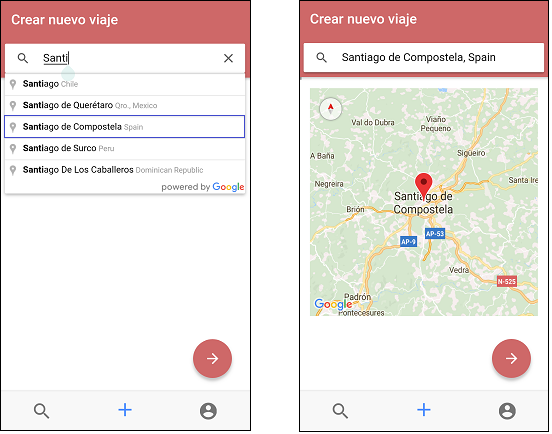
\includegraphics[
   keepaspectratio=true
]{./11_Apendice/Apendice_B/img/Ionic-4-AddRoute.png}
\caption{Pantalla acceso - Aplicación móvil.}
\end{figure}


La pantalla para crear rutas ofrecerá, en la parte superior, un buscador de ciudades. Al buscar una ciudad, el sistema ayudará autocompletando con las ciudades disponibles. Al seleccionar una de ellas, se mostrará un mapa, indicando la ubicación geográfica de dicha ciudad.

Haciendo click en la flecha de la parte inferior de la pantalla, se da de alta ruta en el sistema.

\newpage
\subsubsection*{Mis Datos}







\newpage
\section{Manual de usario aplicación web}

\subsection{Acceso a la aplicación}

Tanto la aplicación web de usuario como la aplicación web de administración tendrán el mismo punto de acceso, que será el siguiente:

\begin{figure}[H]
\centering
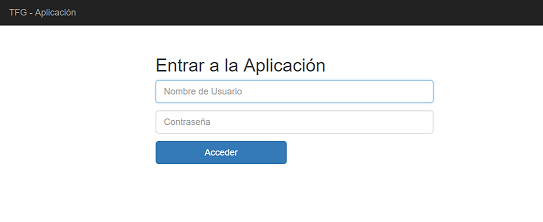
\includegraphics[
   keepaspectratio=true
]{./11_Apendice/Apendice_B/img/WebLogin.png}
\caption{Pantalla acceso - Aplicación web.}
\end{figure}

Se mostrará un pequeño formulario en el que será necesario indicar usuario y contraseña para poder acceder a la aplicación. En función del rol del usuario, se accederá al panel de administración o a la propia aplicación de usuario. 

\subsection{Aplicación de usuario}

\subsubsection*{Pantalla principal}
Si se accede a la aplicación de usuario se mostrará la siguiente pantalla:

\begin{figure}[H]
\centering
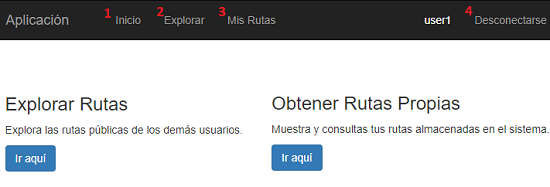
\includegraphics[
   keepaspectratio=true
]{./11_Apendice/Apendice_B/img/WebIndex.png}
\caption{Pantalla principal - Aplicación usuario}
\end{figure}

La barra de navegación será fija para todas las pantallas de la aplicación de usuario y estará formada por:

\begin{itemize}
	\item \textbf{1 - \textit{Inicio}}. Lleva al usuario a esta página.
	\item \textbf{2 - \textit{Explorar}}. Dirige al usuario a la pantalla donde podrá ezplorar las rutas, de los demás usuarios, existentes en la aplicación.
	\item \textbf{3 - \textit{Mis Rutas}}. Dirige al usuario a la pantalla donde podrá consultar las rutas creadas por él mismo.
	\item \textbf{4 - \textit{Desconectarse}}. Permite al usuario desloguearse de la aplicación. Al lado, aparece el nombre de usuario que está actualmente conectado.
\end{itemize}
	
	
En el cuerpo de la página aparecen detalladas las funcionalidades que puede realizar el usuario. En este caso, esas funcionalidades son las mismas que se encuentran en los puntos 2 y 3 de la barra de navegación, \textit{Explorar} y \textit{Mis Rutas}, respectivamente.


\subsubsection*{Explorar rutas}
\begin{figure}[H]
\centering
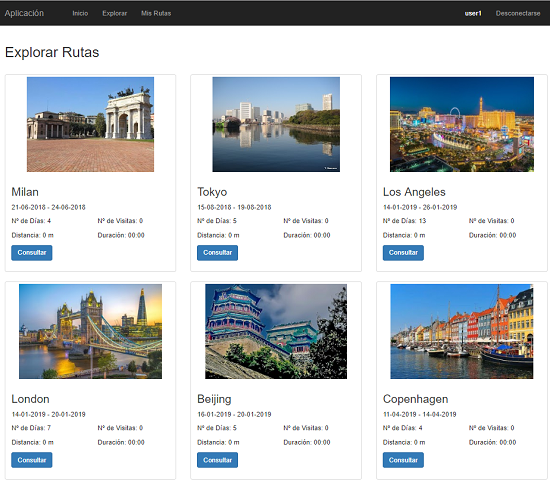
\includegraphics[
   keepaspectratio=true
]{./11_Apendice/Apendice_B/img/WebExploreRoutes.png}
\caption{Pantalla explorar rutas - Aplicación usuario}
\end{figure}

La pantalla de explorar rutas permitirá al usuario obtener las rutas públicas creadas por los demás usuarios de la aplicación. Indicará un listado de las rutas con una pequeña información sobre cada una ellas. Cada ruta incluirá la opción de consultar, que permitirá acceder a la vista de detalles. 

Esta pantalla sigue, visualmente, un estilo similar a la pantalla de \textit{Mis Rutas}, que veremos a continuación más detalladamente. 


\subsubsection*{Mis rutas}

Dentro de la página \textit{Mis Rutas}, el usuario podrá obtener las rutas creadas por él, clasificadas en función de su estado.

\begin{figure}[H]
\centering
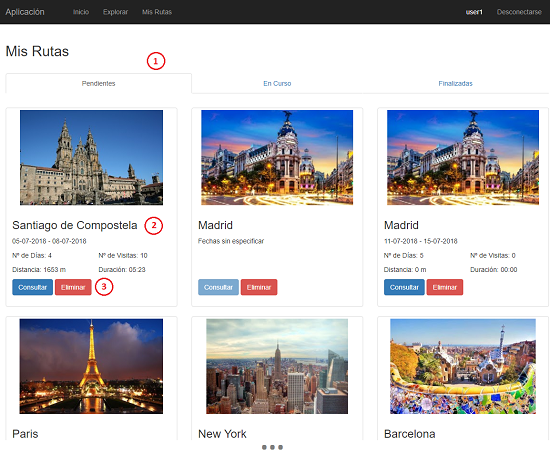
\includegraphics[
   keepaspectratio=true
]{./11_Apendice/Apendice_B/img/WebMyRoutes.png}
\caption{Pantalla mis rutas - Aplicación usuario}
\end{figure}

\begin{itemize}
	\item \textbf{Zona 1.} Selector que permite alternar entre las rutas, clasificadas por los diferentes estados en los que se encuentran.
	\item \textbf{Zona 2.} Bloque que representa la información básica de la ruta. Incluye foto, nombre de la ciudad, fechas, número de días, número de visitas asignadas y distancia y duración totales.
	\item \textbf{Zona 3.} Acciones a realizar sobre determinada ruta.
	\begin{itemize}
		\item Si el usuario selecciona \textit{Eliminar}, se mostrará una alerta, indicando al usuario si desea confirmar o no la acción solicitada.
		\begin{figure}[H]
			\centering
			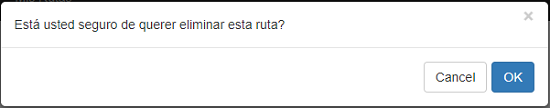
\includegraphics[
			   keepaspectratio=true
			]{./11_Apendice/Apendice_B/img/WebMyRoutesDelete.png}
			\caption{Pantalla eliminar ruta - Aplicación usuario}
		\end{figure}


			
		\item Si el usuario selecciona \textit{Consultar}, el sistema lo dirigirá a la pantalla de \textit{Detalles}, donde podrá obtener la información, detallada por días, de la ruta seleccionada.
	\end{itemize}			
\end{itemize}


\subsubsection*{Detalles ruta}
\begin{figure}[H]
\centering
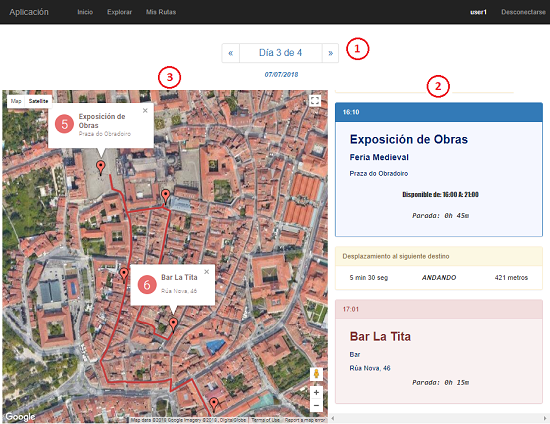
\includegraphics[
	keepaspectratio=true
]{./11_Apendice/Apendice_B/img/WebDetailRoute.png}
\caption{Pantalla detalles ruta - Aplicación usuario}
\end{figure}

En la página de detalles de la ruta tenemos tres zonas diferenciadas:

\begin{itemize}
	\item \textbf{Zona 1. }Selector que permite navegar por los días de la ruta.
	\item \textbf{Zona 2. }Listado, por orden,con los lugares a visitar en determinado día. Cada visita incluye el tiempo de llegada y una pequeña descripción con el nombre del lugar o evento, dirección y tiempo de parada. Se hace distinción por colores, en azul se muestran las visitas a eventos, en rojo las visitas a lugares y en amarilla se indica la información de distancia y tiempo entre cada lugar.
	\item \textbf{Zona 3. }Mapa en el que se muestran las visitas del listado anterior. Haciendo click en cada marca, se abre una ventana de información, en la que se indica el orden de que ocupa dicha visita en la ruta, el nombre y la dirección. Al tratarse de un mapa de Google, se puede interactuar con las funcionalidades que este ofrece, como son la vista en satélite o en mapa, hacer uso del StreetView, entre otras.
\end{itemize}


\subsection{Panel de administración}

\subsubsection*{Barra de navegación}

\begin{figure}[H]
\centering
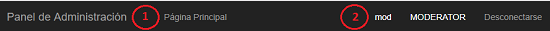
\includegraphics[
   keepaspectratio=true
]{./11_Apendice/Apendice_B/img/WebPanelNavBar.png}
\caption{Barra de navegación - Panel de administración}
\end{figure}

La barra de navegación está formada por:

\begin{itemize}
	\item \textbf{1 - Página principal} Dirige al usuario a la página principal.
	\item \textbf{2 - Información de usuario}. Se mostrará el nombre del usuario conectado junto al rol que desempeña. A la derecha de todo se incluye la opción para desconectarse de la aplicación.
\end{itemize}


\subsubsection*{Pantalla principal}
Si el usuario que accede a la aplicación, tiene rol de gestor de eventos o de administrador se mostrarán, respectivamente, las siguiente pantallas en función del rol.

\begin{figure}[H]
\centering
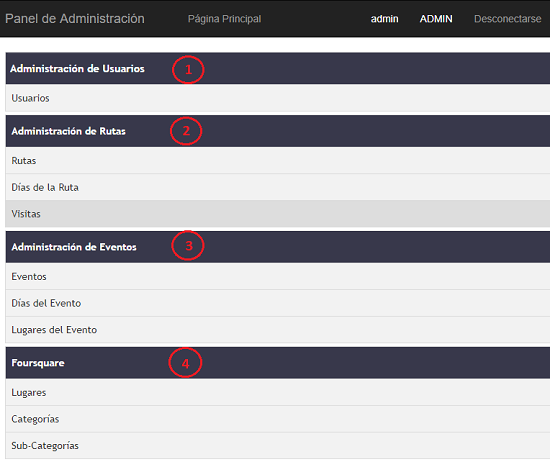
\includegraphics[
   keepaspectratio=true
]{./11_Apendice/Apendice_B/img/WebPanelIndexAdmin.png}
\caption{Pantalla principal administrador - Panel de administración}
\end{figure}


\begin{figure}[H]
\centering
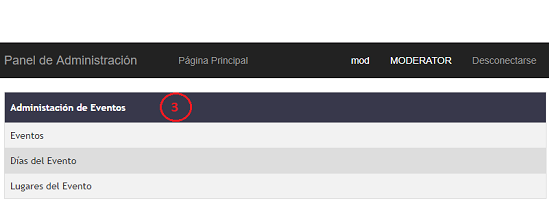
\includegraphics[
   keepaspectratio=true
]{./11_Apendice/Apendice_B/img/WebPanelIndexMod.png}
\caption{Pantalla principal gestor de eventos - Panel de administración}
\end{figure}

En las figuras se diferencian las siguientes zonas.

\begin{itemize}
	\item \textbf{Zona 1. }Redirige al usuario a la administración de usuarios. Está formada por la gestión de la entidad Usuarios.
	\item \textbf{Zona 2. }Redirige al usuario a la administración de las rutas. Está formada por rutas, días y visitas.
	\item \textbf{Zona 3. }Redirige al usuario a la administración de los eventos. Está formada por eventos, días y lugares de evento. Está funcionalidad es la única ofrecida a los usuarios con rol de gestor de eventos.
	\item \textbf{Zona 4. }Redirige al usuario a la gestión de datos de Foursquare. Está formada por los lugares, categorías y subcategorías obtenidas de está fuente externa.
\end{itemize}


\subsubsection*{Pantalla administración usuarios}
Se muestran las entidades que forman la administración de usuarios. En este caso, los usuarios están gestionados mediante una única entidad. Si hubiese más entidades involucradas en dicha gestión aparecerían en pantalla en forma de listado.

\begin{figure}[H]
\centering
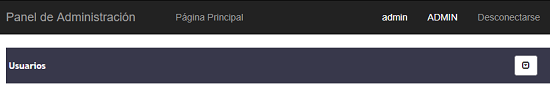
\includegraphics[
   keepaspectratio=true
]{./11_Apendice/Apendice_B/img/WebPanelUsuarios1.png}
\caption{Pantalla administración usuarios - Panel de administración}
\end{figure}

Haciendo click sobre el botón que aparece la derecha de la entidad, se mostrarán los correspondientes datos almacenados. Se mostrarán en formato tabla, siendo las columnas los atributos de la entidad.


\begin{figure}[H]
\centering
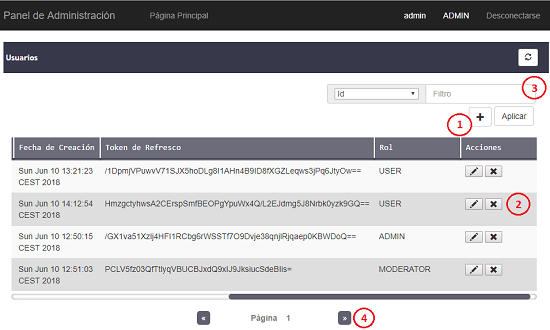
\includegraphics[
   keepaspectratio=true
]{./11_Apendice/Apendice_B/img/WebPanelUsuarios2.png}
\caption{Pantalla administración usuarios - Usuarios - Panel de administración}
\end{figure}

En la figura se diferencian cuatro zonas.


\begin{itemize}
	
	\item \textbf{Zona 1. }Botón que permite dar de alta un nuevo elemento a la entidad. Muestra la siguiente ventana emergente con el formulario a cubrir.
	
\begin{figure}[H]
\centering
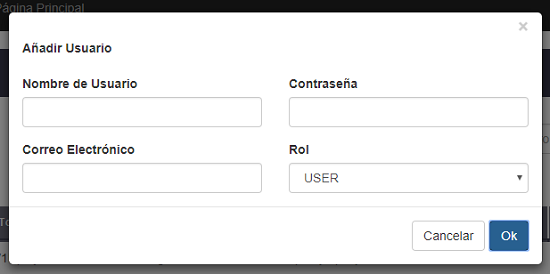
\includegraphics[
   keepaspectratio=true
]{./11_Apendice/Apendice_B/img/WebPanelUsuariosAdd.png}
\caption{Pantalla añadir usuarios - Panel de administración}
\end{figure}

El administrador indicará los datos necesarios y confirmará la acción.
	
	\item \textbf{Zona 2. }Muestra el conjunto de acciones a realizar sobre cada elemento de la tabla. Incluye:
	\begin{itemize}
		\item \textbf{Editar. }Botón con el icono de un lápiz. Muestra una ventana con los datos de dicho elemento, permitiendo realizar modificaciones sobre ellos. Los campos ensombrecidos no pueden ser modificados.
		
		\begin{figure}[H]
		\centering
		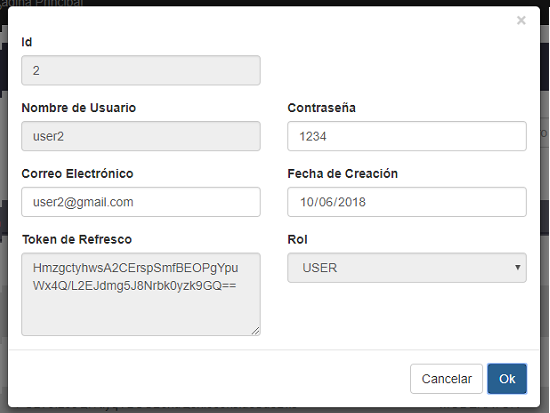
\includegraphics[
   		keepaspectratio=true
		]{./11_Apendice/Apendice_B/img/WebPanelUsuariosEdit.png}
		\caption{Pantalla añadir usuarios - Panel de administración}
		\end{figure}
		
		\item \textbf{Eliminar. }Icono con el botón de una aspa. Muestra una ventana pidiendo confirmación para eliminar dicho elemento.
		\begin{figure}[H]
		\centering
		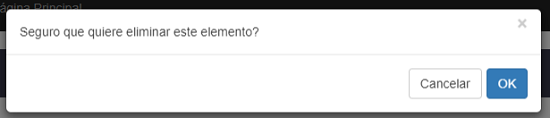
\includegraphics[
   		keepaspectratio=true
		]{./11_Apendice/Apendice_B/img/WebPanelUsuariosDel.png}
		\caption{Pantalla añadir usuarios - Panel de administración}
		\end{figure}
	\end{itemize}		
	
	\item \textbf{Zona 3. }Formada por un selector, un input y un botón de \textit{Aplicar}. En el selector se selecciona el atributo de la entidad sobre el cual se aplicará un filtro, en el input se indicará el valor por el que filtrar y accionando el botón se aplicará dicho filtro sobre la tabla.
	
	\item \textbf{Zona 4. }Indica la paginación de la tabla. Haciendo uso de las flechas, adelante y atrás, se podrán obtener los datos de la entidad de forma paginada.
\end{itemize}


